\section{Programación paralela}

\begin{ejercicio}
    Un programa tarda $40$ s en ejecutarse en un multiprocesador. Durante un 20\% de ese tiempo se
    ha ejecutado en cuatro procesadores; durante un 60\%, en tres; y durante el 20\% restante, en un procesador
    (consideramos que se ha distribuido la carga de trabajo por igual entre los procesadores que colaboran en la
    ejecución en cada momento, despreciamos sobrecarga).
    \begin{enumerate}
        \item ¿Cuánto tiempo tardaría en ejecutarse el programa
        en un único procesador?
        \item ¿Cuál es la ganancia en velocidad obtenida con respecto al tiempo de ejecución
        secuencial?
        \item ¿Cuál es la ganancia en eficiencia obtenida con respecto al tiempo de ejecución
        secuencial?
    \end{enumerate}

    Por el enunciado, tenemos que:
        \begin{gather*}
            T_P = 40 \text{seg.} \\
            T_O(p) = 0 \\
            T_p(p) = T_C(p) + \cancelto{0}{T_O(p)} = T_C(p)
        \end{gather*}
    \begin{enumerate}
        \item
        % // TODO: Incluir una foto con esto en un gráfico (eje x: tiempo, y: nº procesadores)
        Gracias al enunciado, deducimos que desde tiempo 0 hasta $0.2T_P$ se usan 4 procesadores. Desde $0.2T_P$ hasta $0.8T_P$ se usan 3 y desde $0.8T_P$ hasta el final, un único procesador.

        En un único procesador, tendríamos que ejecutar de forma secuencial el código correspondiente a los 4 procesadores (cada uno de $0.2T_P$, luego tendríamos $4\cdot 0.2T_P$), luego a los tres procesadores (cada uno de $0.6T_P$, luego $3\cdot 0.6T_P$) y por último la parte que no es paralelizable (de $0.2T_P$).
        \begin{equation*}
            T_S = 4\cdot 0.2T_P + 3\cdot 0.6T_P + 0.2T_P = 2.8T_P = 2.8 \cdot 40= 112 \text{seg}
        \end{equation*}

        \item
        \begin{equation*}
            S(4) = \dfrac{T_S}{T_P(4)} = \dfrac{2.8\cancel{T_P}}{\cancel{T_P}} = 2.8 
        \end{equation*}

        Recordamos que la ganancia máxima que podemos obtener es de:
        \begin{equation*}
            S(p) = \dfrac{T_S}{T_P(p)} = \dfrac{\cancel{T_S}}{\nicefrac{\cancel{T_S}}{p}} = p
        \end{equation*}
        Mientras que la menor es de:
        \begin{equation*}
            S(p) = \dfrac{T_S}{T_P(p)} = \dfrac{T_S}{T_S} = 1
        \end{equation*}

        Al ser $1 < 2.8 < 4$, podemos intuir que hemos calculado bien la solución.

        \item
        Calculamos la eficiencia:
        \begin{equation*}
            E(p) = \dfrac{\text{Prestaciones}(p)}{p\cdot \text{Prestaciones}(1)} = \dfrac{S(p)}{p} = \dfrac{2.8}{4} = 0.7
        \end{equation*}

        Recordamos que las eficiencias máxima y mínima son:
        \begin{align*}
            E = \dfrac{S}{p} &= \dfrac{p}{p} = 1 \\
            &= \dfrac{1}{p}
        \end{align*}
        Y tenemos que $\nicefrac{1}{4} = 0.25 < 0.7 < 1$ 
        
    \end{enumerate}
\end{ejercicio}

\begin{ejercicio}
    Un programa tarda $20$ s en ejecutarse en un procesador $P_1$, y requiere $30$ s en otro procesador
    $P_2$. Si se dispone de los dos procesadores para la ejecución del programa (despreciamos sobrecarga):
    \begin{enumerate}
        \item ¿Qué tiempo tarda en ejecutarse el programa si la carga de trabajo se distribuye por igual entre los
        procesadores $P_1$ y $P_2$?
        \item ¿Qué distribución de carga entre los dos procesadores $P_1$ y $P_2$ permite el menor tiempo de
        ejecución utilizando los dos procesadores en paralelo? ¿Cuál es este tiempo?
    \end{enumerate}


    \begin{align*}
        T_S^{P_1} &= 20 \text{\ seg} \\
        T_S^{P_2} &= 30 \text{\ seg} \\
        T_O(p) &= 0
    \end{align*}
    Luego tendremos que $T_P(p) = T_C(p) + \cancelto{0}{T_O(p)} = T_C(p)$.

    \begin{enumerate}
        \item 
            Si a los dos le asignamos la mitad del trabajo, tendremos que el procesasdor 1 tarda $\nicefrac{1}{2}\cdot 20 = 10$ segundos, mientras que para el procesador 2, tendremos $\nicefrac{1}{2}\cdot 30 = 15$ segundos. Por tanto:
            \begin{equation*}
                T_P^{P_1, P_2}\left(\frac{1}{2}, \frac{1}{2}\right) = \max\left\{T_S^{P_1}\left(\frac{1}{2}\right), T_S^{P_2}\left(\frac{1}{2}\right)\right\} = \max\{10, 15\} = 15 \text{\ seg}
            \end{equation*}

        \item 
        Repartimos el trabajo de forma que al procesador 1 le asignamos una fracción de trabajo de $x$, por lo que al procesador 2 le tendremos que asignar una carga de $1-x$. Para obtener los mejores tiempos, imponemos que:
        \begin{align*}
            T_S^{P_1}(x) &= T_S^{P_2}(1-x) \\
            x\cdot 20 &= (1-x)\cdot 30 \\
            2x = 3-3x &\Longrightarrow 5x=3 \Longrightarrow x = \frac{3}{5}
        \end{align*}
        Por tanto, tendremos un tiempo de ejecución de:
        \begin{equation*}
            20\cdot \frac{3}{5} = \frac{2}{5}\cdot 30 = 12 \text{\ seg}
        \end{equation*}
    \end{enumerate}

    

\end{ejercicio}

\begin{ejercicio}
    ¿Cuál es fracción de código paralelo de un programa secuencial que, ejecutado en paralelo en 8
    procesadores, tarda un tiempo de 100 ns, durante 50ns utiliza un único procesador y durante otros 50 ns
    utiliza 8 procesadores (distribuyendo la carga de trabajo por igual entre los procesadores)?\\

    Suponiendo que el tiempo de sobrecarga es despreciable (ya que si no no podríamos dar ninguna solución):

    El enunciado nos dice que tenemos un código que en 8 procesadores tarda 100 ns: 50 de los cuales se realiza en un único de procesador y otros 50 ns en los que se reparte eltrabajo por igual entre los 8 procesadores. Por tanto, si lo ejecutásemos en un único procesador, primero deberíamos ejecutar los 50 ns del código no paralelizable y posteriormente deberiamos realizar 8 veces (una por cada procesador) cada parte de 50 ns, teniendo así que ejecutar un código de $(1 + 8)\cdot 50$ ns, de los cuales podemos paralelizar $8\cdot 50$ ns. Por tanto, la fracción de código paralelo es de $\nicefrac{8}{9}$, ya que de 9 partes de código podemos paralelizar 8.
\end{ejercicio}

\begin{ejercicio}
    Un 25\% de un programa no se puede paralelizar, el resto se puede distribuir por igual entre
    cualquier número de procesadores. ¿Cuál es el máximo valor de ganancia de velocidad que se podría
    conseguir al paralelizarlo en $p$ procesadores, y con infinitos? ¿A partir de cuál número de procesadores se
    podrían conseguir ganancias mayores o iguales que 2?\\

    El máximo valor de ganancia que podemos obtener resulta cuando el tiempo de sobrecarga es despreciable:
    \begin{equation*}
        T_P(p) = T_C(p) + \cancelto{0}{T_O(p)}
    \end{equation*}
    Dado que un 25\% del programa no puede paralelizarse, tenemos que $f=\nicefrac{1}{4}$. Por tanto, podemos calcular el tiempo de código paralelo en función del tiempo de código secuencial:
    \begin{equation*}
        T_P(p) = T_C(p) = f\cdot T_S + \left(\dfrac{1-f}{p}\right)T_S
    \end{equation*}
    Con el que calculamos la ganancia:
    \begin{equation*}
        S(p) = \dfrac{T_S}{T_P(p)} = \dfrac{T_S}{f\cdot T_S + \left(\dfrac{1-f}{p}\right)T_S} = \dfrac{1}{f+\dfrac{1-f}{p}} = \dfrac{1}{\dfrac{1}{4}+\dfrac{3}{4p}} = \dfrac{4p}{p+3}
    \end{equation*}
    Es la mayor ganancia que podemos obtener al paralelizarlo en $p$ procesadores. Con infinitos:
    \begin{equation*}
        \lim_{p\to\infty}S(p) = \lim_{p\to\infty}\dfrac{4p}{p+3} = 4
    \end{equation*}
    Finalmente, nos preguntamos por el número $p$ de procesadores necesarios para conseguir ganancias mayores o iguales que 2:
    \begin{equation*}
        S(p) = \dfrac{4p}{p+3} \geq 2 \Longleftrightarrow 4p\geq 2p+6\Longleftrightarrow 2p\geq 6 \Longleftrightarrow p\geq 3
    \end{equation*}
    Por lo que necesitamos 3 procesadores o más para obtener una ganancia mayor que 2.
\end{ejercicio}

\begin{ejercicio}\label{ej:2.5}
    
    En la Figura~\ref{fig:Grafo_2.5}, se presenta el grafo de dependencia entre tareas para una aplicación.
    La figura muestra la fracción del tiempo de ejecución secuencial que la aplicación tarda en ejecutar grupos de tareas del grafo.
    Suponiendo un tiempo de ejecución secuencial de 60 s, que las tareas no se pueden dividir en tareas de menor granularidad y
    que el tiempo de comunicación es desprecible, obtener el tiempo de ejecución en paralelo y la ganancia en velocidad en un computador con:
    \begin{enumerate}
        \item 4 procesadores.
        \item 2 procesadores.
    \end{enumerate}
    \begin{figure}
        \centering
        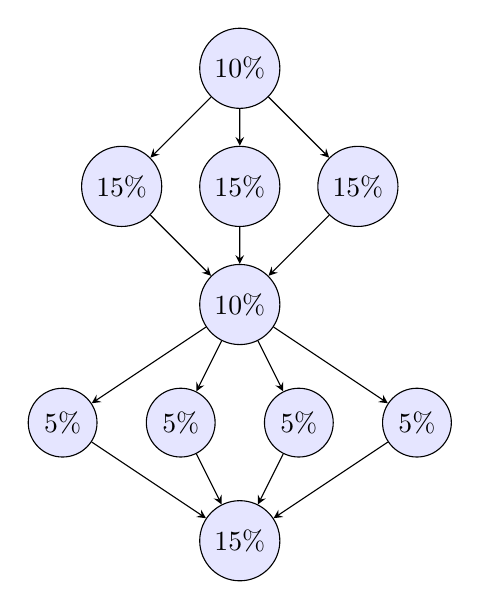
\begin{tikzpicture}[
            every node/.style={circle, draw, fill=blue!10},
            level 1/.style={sibling distance=1.5cm},
            level 2/.style={sibling distance=1cm},
            level 3/.style={sibling distance=1cm},
            level 4/.style={sibling distance=1cm},
            level distance=1.5cm,
            sibling distance=2.5cm,
            edge from parent/.style={draw,-stealth}
            ]
            \node (topnode) at (0,5) {10\%} 
            child{node{15\%}}
            child{node{15\%}}
            child{node{15\%}}
            ;
    
            \node (middlenode) at (0,2) {10\%}
            child{node{5\%}}
            child{node{5\%}}
            child{node{5\%}}
            child{node{5\%}}
            ;
    
            \node(bottomnode) at (0,-1) {15\%};
    
            \foreach \x in {1,2,3,4}{
                \draw[-stealth] (middlenode-\x) -- (bottomnode);
            }
    
            \foreach \x in {1,2,3}{
                \draw[-stealth] (topnode-\x) -- (middlenode);
            }
        \end{tikzpicture}
        \caption{Grafo de tareas del Ejercicio~\ref{ej:2.5}}
        \label{fig:Grafo_2.5}
    \end{figure}

    \begin{align*}
        T_S &= 60 \text{\ seg} \\
        T_O(p) &= 0
    \end{align*}
    Luego tenemos que $T_P(p) = T_C(p) + \cancelto{0}{T_O(p)} = T_C(p)$.

    Numeramos las tareas (los nodos) de arriba a abajo y de izquierda a derecha. 
    Observando el gráfico, vemos que el número máximo de nodos en el mismo nivel es 4, luego el número máximo de procesadores (cores) que podremos usar como máximo será de 4.

    \begin{enumerate}
        \item 
            \begin{itemize}
                \item La tarea 1 tendrá un tiempo de ejecución de $0.1T_S$.
                \item Posteriormente, tenemos a las tareas 2, 3 y 4, con tiempos de ejecución $0.15T_S$.
                \item Además, la tarea 5, con tiempo $0.1T_S$.
                \item Las tareas 6, 7, 8 y 9 con $0.05T_S$.
                \item Por último, la tarea 10, con $0.15T_S$
            \end{itemize}

            \begin{equation*}
                T_P(4) = 0.1T_S + 0.15T_S + 0.1T_S + 0.05T_S + 0.15T_S = 0.55T_S = 0.55\cdot 60 = 33 \text{\ seg}
            \end{equation*}

            Calculamos la ganancia:
            \begin{equation*}
                S(4) = \dfrac{T_S}{T_P(4)} = \dfrac{T_S}{0.55T_S} = \dfrac{60}{33} = \dfrac{20}{11} = 1.82 < 4
            \end{equation*}
            Siendo 4 la ganancia máxima esperable (al usar 4 procesadores).

        \item 
            \begin{itemize}
                \item La tarea 1 tendrá un tiempo de ejecución de $0.1T_S$, al igual que en 4 procesdores.
                \item En este caso, las tareas 2, 3 y 4 no pueden ejecutarse en paralelo todas a la vez, tendremos que ejecutar primer la 2 y la 3 ($0.15T_S$) y después la 4 ($0.15T_S$).
                \item La tarea 5 con $0.10T_S$.
                \item La 6 y 7 con $0.05T_S$ y las 8, 9 con $0.05T_S$.
                \item Y por último la 10 con $0.15T_S$
            \end{itemize}

            \begin{equation*}
                T_P(2) = 0.1T_S + 2\cdot 0.15T_S + 0.1T_S + 2\cdot 0.05 T_S + 0.15 T_S = 0.75 \cdot 60 = 45 \text{\ seg}
            \end{equation*}

            \begin{equation*}
                S(2) = \dfrac{T_S}{T_P(2)} = \dfrac{\cancel{T_S}}{0.75\cdot \cancel{T_S}} = \frac{1}{0.75} = \frac{4}{3} \approx 1.333 < 2
            \end{equation*}
        
    \end{enumerate}
    

\end{ejercicio}


\begin{ejercicio} \label{ej:2.6}
    Un programa se ha conseguido dividir en 10 tareas. El orden de precedencia entre las tareas se
    muestra con el grafo dirigido de la Figura~\ref{fig:Grafo_2.6}. La ejecución de estas tareas en un procesador supone un tiempo de 2 sg.
    El 10\% de ese tiempo es debido a la ejecución de la tarea 1; el 15\% a la ejecución de la tarea 2; otro 15\% a la ejecución de 3;
    cada tarea 4, 5, 6 o 7 supone el 9\%; un 8\% supone la tarea 8; la tarea 9 un 10\%; por último, la tarea 10 supone un 6\%.
    Se dispone de una arquitectura con 8 procesadores para ejecutar la aplicación. Consideramos que el tiempo de comunicación se puede despreciar.
    \begin{enumerate}
        \item ¿Qué tiempo tarda en ejecutarse el programa en paralelo?
        \item ¿Qué ganancia en velocidad se obtiene con respecto a su ejecución secuencial?
    \end{enumerate}
    \begin{figure}
        \centering
        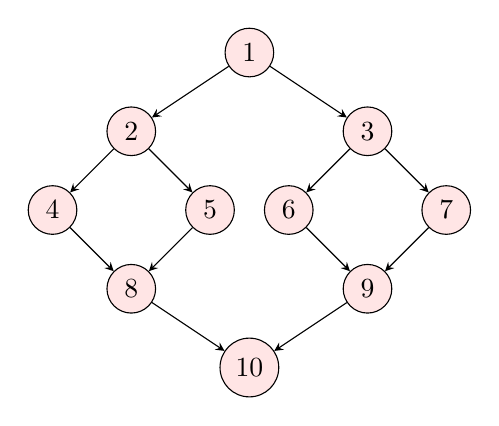
\begin{tikzpicture}[
            every node/.style={circle, draw, fill=red!10},
            level 1/.style={sibling distance=3cm},
            level 2/.style={sibling distance=2cm},
            level 3/.style={sibling distance=2.5cm},
            level 4/.style={sibling distance=1cm},
            level distance=1cm,
            sibling distance=3cm,
            edge from parent/.style={draw,-stealth}]

            \node (topnode) at (0,4) {1} 
                child { node {2}
                    child { node {4}}
                    child { node {5}}
                }
                child { node {3}
                    child { node {6}}
                    child { node {7}}
                }
            ;

            \node(bottomnode) at (0,0) {10} [grow=up]
                child[edge from parent/.style={draw,stealth-}] { node {9}}
                child[edge from parent/.style={draw,stealth-}] { node {8}}
            ;

            \foreach \i in {1,2}{
                \draw[-stealth] (topnode-1-\i) -- (bottomnode-2);
            }

            \foreach \i in {1,2}{
                \draw[-stealth] (topnode-2-\i) -- (bottomnode-1);
            }
        \end{tikzpicture}
        \caption{Grafo de tareas del Ejercicio~\ref{ej:2.6}}
        \label{fig:Grafo_2.6}
    \end{figure}

    % todo esto lo hizo la tia en clase, ni puta idea del ejercicio
    %Vamos a plantear varios flujos de ejecución. % // TODO:(pedir a Irina). 
    %Vemos las comunicaciones que suponen cada uno de los caminos.
    %Tengamos en cuenta que los nodos en la misma altura tienen el mismo tiempo de ejecución. Para la hora de calcular los costes de las comunicaciones.
%
    %\begin{itemize}
        %\item Vamos a asignar las tareas 1, 2, 4, 8 y 10 al procesadsor 1.
        %\item Las tareas 3, 6 y 9 al 2.
        %\item La 5 al 3.
        %\item La 7 al 4.
    %\end{itemize}
%
    %\begin{equation*}
        %T_P(4) = T_C(4) + T_O(4)
    %\end{equation*}
    %10 es la última, que necesita de 8 y 9. 9 requiere de la finalización de 6 y 7, de donde 7 requiere la finalización de 3.
%
    %Tenemos varios caminos de datos que llegan a 10.
    %Obtenemos 4 comunicaciones.
%
    %\begin{itemize}
        %\item Las tareas 1, 2 y 4 al proesador 1.
        %\item Las 3 y 6 al 2.
        %\item Las 5 y 8 al 3.
        %\item Las 7, 9 y 10 al 4.
    %\end{itemize}
    %Tenemos 2 comunicaciones % // TODO: preguntar a JJ a la hora de redactar
    

\end{ejercicio}

\begin{ejercicio}
    Se quiere paralelizar el siguiente trozo de código:
    \begin{minted}[xleftmargin=3cm]{c++}
//  {Cálculos antes del bucle}
for( i=0; i<w; i++) {
    // Código para i
}
// {cálculos después del bucle}
    \end{minted}
    Los cálculos antes y después del bucle suponen un tiempo de $t_1$ y $t_2$, respectivamente.
    Una iteración del ciclo supone un tiempo $t_i$. En la ejecución paralela, la inicialización de $p$ procesos supone un tiempo
    $k_1p$ ($k_1$ constante), los procesos se comunican y se sincronizan, lo que supone un tiempo $k_2p$ ($k_2$ constante); $k_1p+k_2p$
    constituyen la sobrecarga.
    \begin{enumerate}
        \item Obtener una expresión para el tiempo de ejecución paralela del trozo de código en $p$ procesadores ($T_p$).
        \item Obtener una expresión para la ganancia en velocidad de la ejecución paralela con respecto a una ejecución secuencial ($S_p$).
        \item ¿Tiene el tiempo $T_p$ con respecto a $p$ una característica lineal o puede presentar algún mínimo? ¿Por qué? En caso de presentar un mínimo, ¿para qué número de procesadores $p$ se alcanza?
    \end{enumerate}

    \begin{enumerate}
        \item Para obtener una expresión del tiempo de ejecución en paralelo del trozo de código en $p$ procesadores, necesitamos:
            \begin{equation*}
                T_P(p) = T_C(p) + T_O(p)
            \end{equation*}
            Sabemos ya que $T_O(p) = p(k_1 + k_2)$, mientras que razonamos el valor de $T_C(p)$:

            Tenemos una sección de código no paralelizable (los cálculos que se realizan antes del bucle y los que se realizan después), que tiene un costo $t_1+t_2$. Además, contamos con $w$ iteraciones de un código paralelizable, cada una de ellas con un costo $t_i$. Por tanto, este código tardaría $w\cdot t_i$ en un solo procesador. Sin embargo, al disponer de $p$ procesadores, este tiempo disminuye a $\frac{w\cdot t_i}{p}$. Resumiendo:
            \begin{equation*}
                T_C(p) = t_1 + t_2 + \dfrac{w\cdot t_i}{p}
            \end{equation*}
            En consecuencia:
            \begin{equation*}
                T_P(p) = t_1 + t_2 + \dfrac{w\cdot t_i}{p} + p(k_1+k_2)
            \end{equation*}
        \item Para el cálculo de la ganancia en velocidad, debemos primero calcular el tiempo de ejecución secuencial del programa. Por un razonamiento análogo, tenemos que ejecutar la parte del código no paralelizable (con un tiempo de $t_1 + t_2$) y las $w$ iteraciones del bucle, cada una de tiempo $t_i$:
            \begin{equation*}
                T_S = t_1 + t_2 + w\cdot t_i
            \end{equation*}
            De donde:
            \begin{equation*}
                S(p) = \dfrac{T_S}{T_P(p)} = \dfrac{t_1 + t_2 + w\cdot t_i}{t_1 + t_2 + \dfrac{w\cdot t_i}{p} + p(k_1 + k_2)}
            \end{equation*}

        \item Para terminar con el ejercicio, vamos ahora a estudiar si $T_P(p)$ tiene mínimo. Calculamos sus puntos críticos:
            \begin{equation*}
                T_P'(p) = \dfrac{-wt_i}{p^2} + (k_1+k_2)
            \end{equation*}
            \begin{equation*}
                T_P'(p) = 0 \Longleftrightarrow \dfrac{-wt_i}{p^2} + (k_1+k_2) = 0 \Longleftrightarrow \dfrac{w\cdot t_i}{p^2}=k_1 + k_2 \Longleftrightarrow p = \pm \sqrt{\dfrac{w\cdot t_i}{k_1+k_2}}
            \end{equation*}
            Donde descartamos la solución negativa por no tener sentido en este caso. Comprobamos ahora si este punto crítico es un mínimo o un máximo, calculando la segunda derivada de $T_P(p)$:
            \begin{equation*}
                T_P''(p)= \dfrac{2pwt_i}{p^4} = \dfrac{2wt_i}{p^3} > 0
            \end{equation*}
            Luego se trataba de un mínimo, el cual se alcanza en:
            \begin{equation*}
                \left\lceil \sqrt{\dfrac{w\cdot t_i}{k_1+k_2}} \right\rceil \text{\ procesadores}
            \end{equation*}

    \end{enumerate}
\end{ejercicio}

\begin{ejercicio}
    Supongamos que se va a ejecutar en paralelo la suma de $n$ números en una arquitectura con $p$
    procesadores o cores ($p$ y $n$ potencias de dos) utilizando un grafo de dependencias en forma de árbol (divide
    y vencerás) para las tareas.
    \begin{enumerate}
        \item\label{ej:2.8a} Dibujar el grafo de dependencias entre tareas para $n=16$ y $p=8$. Hacer una asignación de tareas
        a procesos.
        \item Obtener el tiempo de cálculo paralelo para cualquier $n$ y $p$ con $n>p$ suponiendo que se tarda una
        unidad de tiempo en realizar una suma.
        \item\label{ej:2.8c} Obtener el tiempo comunicación del algoritmo suponiendo:
        \begin{enumerate}
            \item Que las comunicaciones en un nivel del árbol se pueden realizar en paralelo en un número de unidades de tiempo igual al número de
            datos que recibe o envía un proceso en cada nivel del grafo de tareas (tenga en cuenta la asignación
            de tareas a procesos que ha considerado en el apartado~\ref{ej:2.8a})
            \item Que los procesadores que realizan las tareas de las hojas del árbol tienen acceso sin coste de comunicación a los datos que utilizan
            dichas tareas.
        \end{enumerate}

        \item Suponiendo que el tiempo de sobrecarga coincide con el tiempo de comunicación calculado en el apartado~\ref{ej:2.8c}, obtener la ganancia en prestaciones.
        \item Obtener el número de procesadores para el que se obtiene la máxima ganancia con $n$ números.
    \end{enumerate}

Vamos a sumar $n$ números en $p$ procesadores. 

Dados 4 sumandos $S_0, S_1, S_2, S_3$, combinaríamos $S_0$ con $S_1$ y $S_2$ con $S_3$, combinando finalmente estos dos. Por tanto, dados 4 nodos iniciales, tendríamos 2 comunicaciones. Dados 8, 3. El número de comunicaciones es de $\log_2 p$, siendo $p$ el número de nodos iniciales, que coincide con el número de procesadores.

\begin{equation*}
    T_P(p,n) = T_C(p,n) + T_{C,S}(p,n) = \left(\frac{n}{p}-1\right)\log_2 p + \log_2 p
\end{equation*}
Donde $T_{C,S}(p,n)$ es el tiempo de las comunicaciones ($C$) en paralelo ($S$) del programa que suma $n$ números en $p$ procesadores.
\begin{equation*}
    S(p,n) = \dfrac{T_S(n)}{T_P(n,p)} = \dfrac{n-1}{\left(\frac{n}{p}-1\right)+2\log_2p} 
\end{equation*}

\end{ejercicio}

\begin{ejercicio} \label{ej:2.9}
    Se va a paralelizar un decodificador JPEG en un multiprocesador. Se ha extraído para la aplicación
    el siguiente grafo de tareas que presenta una estructura segmentada (o de flujo de datos):
    \begin{figure}[H]
        \centering
        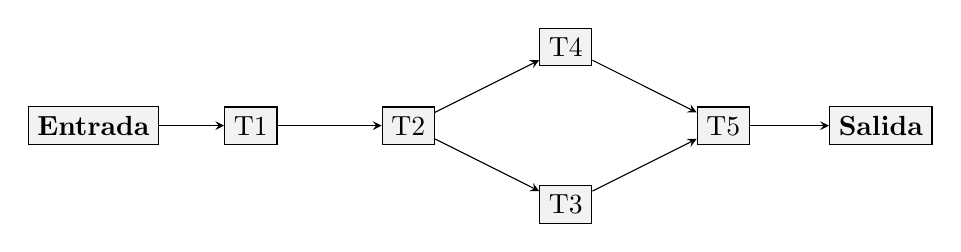
\begin{tikzpicture}[every node/.style={draw, fill=gray!10}, node distance=2cm]
            \node (entrada) [draw] {\textbf{Entrada}};
            \node (T1) [draw, right of=entrada] {T1};
            \node (T2) [draw, right of=T1] {T2};
            \node (T3) [draw, right of=T2, yshift=-1cm] {T3};
            \node (T4) [draw, right of=T2, yshift=1cm] {T4};
            \node (T5) [draw, right of=T4, yshift=-1cm] {T5};
            \node (salida) [draw, right of=T5] {\textbf{Salida}};
            
            \draw[-stealth] (entrada) -- (T1);
            \draw[-stealth] (T1) -- (T2);
            \draw[-stealth] (T2) -- (T3);
            \draw[-stealth] (T2) -- (T4);
            \draw[-stealth] (T3) -- (T5);
            \draw[-stealth] (T4) -- (T5);
            \draw[-stealth] (T5) -- (salida);
        \end{tikzpicture}
        \caption{Segmentación del Ejercicio~\ref{ej:2.9}}
    \end{figure}
    La entrada tenemos que es el bloque de la imagen a decodificar (supone 8x8 pixels de la imagen).
    La salida será el bloque decodificado de 8x8 pixel. Las tareas 1, 2 y 5 se ejecutan en un tiempo igual a $t$,
    mientras que las tareas 3 y 4 suponen $1.5t$. El decodificador JPEG aplica el grafo de tareas de la figura a bloques de la imagen, cada uno de 8x8 píxeles. Si
    se procesa una imagen que se puede dividir en $n$ bloques de 8x8 píxeles, a cada uno de esos $n$ bloques se
    aplica el grafo de tareas de la figura. Obtenga la mayor ganancia en prestaciones que se puede conseguir
    paralelizando el decodificador JPEG en (suponga despreciable el tiempo de comunicación/sincronización):
    \begin{enumerate}
        \item 5 procesadores.
        \item 4 procesadores.
    \end{enumerate}

    En cualquier de los dos casos, la ganancia se tiene que calcular suponiendo que se procesa una imagen con un total de $n$ bloques de 8x8 píxeles.


\begin{enumerate}
    \item
    Contamos con 4 etapas en el cauce.
\begin{table}[H]
    \begin{tabular}{|c|c|c|c|c|c|c|c|c|}
        \hline
        Bloque & Entra 1 & Sale 1 & Entra 2 & Sale 2 & Entra 3 & Sale 3 & Entra 4 & Sale 4 \\
        \hline
        B1 & 0 & t & t & 2t & 2t & 3.5t & 3.5t & 4.5t \\
        B2 & t & 2t & 2t & 3t & 3.5t & 5t & 5t & 6t \\
        B3 & 2t & 3t & 3t & 4t & 5t & 6.5t & 6.5t & 7.5t\\
        \hline
    \end{tabular}
\end{table}
Desde que sale el bloque 1 hasta el bloque 2, transcurren $1.5t$, al igual que desde 2 hasta 3.

\begin{equation*}
    T_P(5) = \underbrace{4.5t}_{B1} + \underbrace{1.5t}_{B2} + \underbrace{1.5t}_{B3} + \cdots + \underbrace{1.5t}_{Bn}
\end{equation*}
\begin{equation*}
    T_P(5) = TLI + (n-1)TEML
\end{equation*}
Donde $TLI$ es el Tiempo de Latencia Inicial y $TEML$ es el Tiempo de la Etapa Más Lenta.

La ganancia:
\begin{equation*}
    S(5,n) = \dfrac{T_S(n)}{T_P(5,n)} = \dfrac{\left(\sum\limits_{i=1}^{5}r_i \right)\cdot n}{TLI + (n-1)TEML}
\end{equation*}
Donde $r_i$ es el tiempo de la tarea $i$, que cuando $n\rightarrow\infty$, tenemos que:
\begin{equation*}
    \lim_{n\to\infty}S(5,n) = \dfrac{\sum\limits_{i=1}^{5}r_i}{TEML} = \dfrac{6t}{1.5t} = 4
\end{equation*}

Vamos a realizar la siguiente asignación:
    \begin{itemize}
        \item La tarea 1 al procesador 1.
        \item La tarea 2 al 2.
        \item Las 3 y la 4 al 3.
        \item La tarea 5 al 4.
    \end{itemize}
    Se trata de una distribución en 4 etapas para segmentación. Así, tenemos $TEML = 1.5t\cdot 2=3t$.

    Sin embargo, con una distribución:
    \begin{itemize}
        \item Las tareas 1 y 2 al procesador 1.
        \item Las 3 y 4 al 2.
        \item La tarea 5 al 3.
    \end{itemize}
    En este caso, tenemos 3 estapas segmentadas. Obtenemos $TEML = t\cdot 2 = 2t$.
    
\end{enumerate}



\end{ejercicio}


\begin{ejercicio}
    Se quiere implementar un programa paralelo para un multicomputador que calcule la siguiente
    expresión para cualquier $x$ (es el polinomio de interpolación de Lagrange):
    $P(x) = \sum\limits_{i=0}^{n} \left(b_i\cdot L_i(x)\right)$, donde:
    \begin{align*}
        L_i(x) &= \frac{(x-a_0) \ldots  (x-{a_{i-1}})(x-{a_{i+1}}) \ldots  (x-a_n)}{k_i}
        = \frac{\prod\limits_{\substack{j=0\\ j\neq i}}^{n} (x-a_j)}{k_i} \qquad i=0,1,\dots,n\\
        k_i &= (a_i-a_0) \ldots  (a_i-a_{i-1})(a_i-a_{i+1}) \ldots  (a_i-a_n)= \prod\limits_{\substack{j=0\\ j\neq i}}^{n} (a_i-a_j) \qquad i=0,1,\dots,n
    \end{align*}

    Inicialmente $k_i$, $a_i$ y $b_i$ se encuentran en el nodo $i$ y $x$ en todos los nodos. Sólo se van a usar funciones de
    comunicación colectivas. Indique cuál es el número mínimo de funciones colectivas que se pueden usar,
    cuáles serían, en qué orden se utilizarían y para qué se usan en cada caso.
\end{ejercicio}

\begin{ejercicio}\label{ej:2.11}~
    \begin{enumerate}
        \item Escriba un programa secuencial con notación algorítmica (podría escribirlo en C) que
        determine si un número de entrada, $x$, es primo o no. El programa imprimirá si es o no primo. Tendrá
        almacenados en un vector, \verb|NP|, los $M$ números primos entre 1 y el máximo valor que puede tener un número
        de entrada al programa.

        \item Escriba una versión paralela del programa anterior para un multicomputador usando un estilo de
        programación paralela de paso de mensajes. El proceso 0 tiene inicialmente el número $x$ y el vector \verb|NP| en su
        memoria e imprimirá en pantalla el resultado. Considere que la herramienta de programanción ofrece
        funciones \verb|send()/receive()| para implementar una comunicación uno-a-uno asíncrona, es decir, con función
        \verb|send(buffer,count,datatype,idproc,group)| no bloqueante y
        \verb|receive(buffer,count,datatype,idproc,group)| bloqueante. En las funciones \verb|send()/receive()| se
        especifica:
        \begin{itemize}
            \item \verb|group|: identificador del grupo de procesos que intervienen en la comunicación.
            \item \verb|idproc|: identificador del proceso al que se envía o del que se recibe.
            \item \verb|buffer|: dirección a partir de la cual se almacenan los datos que se envían o los datos que se
            reciben.
            \item \verb|datatype|: tipo de los datos a enviar o recibir (entero de 32 bits, entero de 64 bits, flotante de 32
            bits, flotante de 64 bits, \dots).
            \item \verb|count|: número de datos a transferir de tipo \verb|datatype|.
        \end{itemize}
    \end{enumerate}
\end{ejercicio}

\begin{ejercicio} \label{ej:2.12}
    Escribir una versión paralela del programa secuencial del ejercicio~\ref{ej:2.11} para un multicomputador
    usando un estilo de programación paralela de paso de mensajes y suponiendo que la herramienta de
    programación ofrece las funciones colectivas de difusión y reducción (escribir primero la versión secuencial). 
    Sólo el proceso 0 imprimirá en pantalla. En la función de difusión,
    \verb|broadcast(buffer,| \verb|count,datatype,| \verb|idproc,group)|, se especifica:
    \begin{itemize}
        \item \verb|group|: identificador del grupo de procesos que intervienen en la comunicación, todos los procesos
        del grupo reciben.
        \item \verb|idproc|: identificador del proceso que envía.
        \item \verb|buffer|: dirección de comienzo en memoria de los datos que difunde \verb|idproc| y que almacenará,
        en todos los procesos del grupo, los datos difundidos.
        \item \verb|datatype|: tipo de los datos a enviar/recibir (entero de 32 bits, entero de 64 bits, flotante de 32
        bits, flotante de 64 bits, \dots).
        \item \verb|count|: número de datos a transferir de tipo \verb|datatype|.
    \end{itemize}
    En la función de reducción, \verb|reduction(sendbuf,| \verb|recvbuf,count,| \verb|datatype,oper,| \verb|idproc,group)|,
    se especifica:
    \begin{itemize}
        \item \verb|group|: identificador del grupo de procesos que intervienen en la comunicación, todos los procesos
        del grupo envían.
        \item \verb|idproc|: identificador del proceso que recibe.
        \item \verb|recvbuf|: dirección en memoria a partir de la cual se almacena el escalar resultado de la reducción
        de todos los componentes de todos los vectores \verb|sendbuf|.
        \item \verb|sendbuf|: dirección en memoria a partir de la cual almacenan todos los procesos del grupo los
        datos de tipo \verb|datatype| a reducir (uno o varios).
        \item \verb|datatype|: tipo de los datos a enviar y recibir (entero de 32 bits, entero de 64 bits, flotante de 32
        bits, flotante de 64 bits, \dots).
        \item \verb|oper|: tipo de operación de reducción. Puede tomar los valores \verb|OR|, \verb|AND|, \verb|ADD|, \verb|MUL|,\verb|MIN|,\verb|MAX|
        \item \verb|count|: número de datos de tipo \verb|datatype|, del buffer \verb|sendbuffer| de cada proceso, que se van a reducir.
    \end{itemize}
\end{ejercicio}

\begin{ejercicio}~
    \begin{enumerate}
        \item\label{ej:2.13a} Escribir una versión paralela del programa paralelo del ejercicio~\ref{ej:2.12} suponiendo que, además de las
        dos funciones colectivas anteriores, se dispone de dispersión y que $M$ es divisible entre el número de
        procesos (escribir primero la versión secuencial). Sólo el proceso 0 imprimirá en pantalla. La función
        \verb|scatter(sendbuf,sendcnt,recvbuf,recvcnt,datatype,idproc,group)| especifica:
        \begin{itemize}
            \item \verb|group|: identificador del grupo de procesos que intervienen en la comunicación, todos los procesos
            del grupo envían.
            \item \verb|idproc|: identificador del proceso que envía.
            \item \verb|recvbuf|: dirección en memoria a partir de la cual se almacenan los datos recibidos.
            \item \verb|sendbuf|: dirección en memoria a partir de la cual almacena el proceso \verb|idproc| los datos a enviar.
            \item \verb|sendtype|: tipo de los datos a enviar y recibir.
            \item \verb|recvcnt|: número de datos de tipo \verb|datatype| a recibir en \verb|recvbuf|.
            \item \verb|sendcnt|: número de datos de tipo \verb|datatype| a enviar.
        \end{itemize}

        \item ¿Qué estructura de procesos/tareas implementa el código paralelo del apartado~\ref{ej:2.13a}? Justifique su respuesta.
    \end{enumerate}
\end{ejercicio}

\begin{ejercicio}
    Escribir una versión paralela del programa secuencial del ejercicio~\ref{ej:2.11} para un multiprocesador
    usando el estilo de programación paralela de variables compartidas; en particular, use OpenMP (escribir
    primero la versión secuencial).
\end{ejercicio}

\subsection{Cuestiones}
\begin{cuestion}
    Indique las diferencias entre OpenMP y MPI.\\

    OpenMP es una API de directivas y funciones, mientras que MPI es una API de funciones. Ambas son herramientas que permiten desarrollar paralelismo. Sin embargo, como hemos ya mencionado en la parte teórica, la abstracción en la que nos sitúa OpenMP es mayor a al que nos provee MPI: mientras que en MPI hemos de preocuparnos de muchos detalles a la hora de implementar el paralelismo, en OpenMP le decimos a la herramienta que realice cierta tarea y ya es el compilador quien se encarga de resolver estos detalles.
\end{cuestion}

\begin{cuestion}
    Ventajas e inconvenientes de una asignación estática de tareas a procesos/threads frente a una asignación dinámica.\\

    La principal desventaja de la asignación dinámica frente a la estática es la necesidad de calcular en cada momento qué asignación de trabajo es la mejor a desarrollar en cada momento: tener en cuenta qué nodos de trabajo se encuentran ocupados y cuales no y dividir el trabajo conforme a ello.

    Como ventajas, podemos destacar dos:
    \begin{itemize}
        \item En caso de una asignación compleja (podemos realizar una asignación estática, pero obtenerla es muy dificultosa), podemos simplemente realizar una asignación dinámica, ahorrando al programador la tarea del cálculo de los trabajos de cada nodo.
        \item Cuando no se conoce el número de tareas que se ejecutarán (por ejemplo, porque depende de un parámetro que se conoce en tiempo de ejecución), no es posible llevar a cabo una asociación estática.
    \end{itemize}
\end{cuestion}

\begin{cuestion}
    ¿Qué se entiende por escalabilidad lineal y por escalabilidad superlineal? Indique las causas por las que se puede obtener una escalabilidad superlineal.\\

    Decimos que un programa que resuelve una aplicación de forma paralela es escalable linealmente cuando su ganancia de velocidad en comparación con el tiempo secuencial resulta en el número de procesadores. Es decir, decimos que una aplicación paralela escala linealmente si:
    \begin{equation*}
        S(p) = p
    \end{equation*}
    Por otra parte, decimos que escala de forma superlineal si:
    \begin{equation*}
        S(p) > p
    \end{equation*}
    Un ejemplo de escalabilidad superlineal es el resultado de aplicar una búsqueda lineal paralela a cierta instancia, de forma que en pocas iteraciones encuentre el elemento buscado gracias a partir el vector para su paralelización, tal y como comentamos en la Sección~\ref{ej:superlineal}.
\end{cuestion}

\begin{cuestion}
    Enuncie la ley de Amdahl en el contexto de procesamiento paralelo.\\

    Dado un código secuencial cuyo tiempo de ejecución suponemos constante en $T_S$ segundos, suponemos que tenemos una fracción $f$ de código no paralelizable y que usamos $p$ procesadores para la fracción de código que sí es paralelizable. En dicho caso, obtendremos una ganancia con $p$ procesadores de a lo sumo:
    \begin{equation*}
        S(p) \leq \dfrac{p}{1+f(p-1)}
    \end{equation*}
\end{cuestion}

\begin{cuestion}
    Deduzca la expresión matemática que se suele utilizar para caracterizar la ley de Gustafson. Defina claramente y sin ambigüedad el punto de partida que va a utilizar para deducir esta expresión y cada una de las etiquetas que utilice. ¿Qué nos quiere decir Gustafson con esta ley?\\

    Supuesto que el tiempo de ejecución de un código paralelo es constante fijado un número $p$ de procesadores en $T_P(p)$, procedemos a calcular el tiempo de ejecución secuencial de dicho programa en función del tiempo de ejecución en paralelo, sabiendo que existe una fracción $f$ de código no paralelizable:
    \begin{equation*}
        T_S = f\cdot T_P(p) + p(1-f)\cdot T_P(p)
    \end{equation*}
    Ya que la fracción de código no paralelizable será la misma. Además, si antes tardábamos $(1-f)T_P(p)$ en ejecutar la parte paralelizable entre $p$ procesadores, si asumimos un reparto equitativo, en un procesador tendremos que hacer $p$ veces este tiempo. De esta forma, calculamos la ganancia:
    \begin{equation*}
        S(p) = \dfrac{T_S}{T_P(p)} = \dfrac{f\cdot \cancel{T_P(p)} + p(1-f)\cancel{T_P(p)}}{\cancel{T_P(p)}} = f+p(1-f)
    \end{equation*}
    Con esta ley, Gustafson nos indica que la ganancia depende de forma lineal del número $p$ de procesadores, con una pendiente de $1-f$, lo que nos indica que, a mayor sea $1-f$ (luego, menor sea $f$), es decir, la parte paralelizable; mayor será la ganancia de velocidad al paralelizar.
\end{cuestion}

\begin{cuestion}
    Deduzca la expresión que caracteriza a la ley de Amdahl. Defina claramente el punto de partida y todas las etiquetas que utilice.\\

    Supuesto que el tiempo de ejecución de un programa en un procesador es constante en $T_S$ segundos y supuesto que pasamos a una versión del programa con código paralelo con $p$ procesadores y una fracción de código no paralelizable $f$. Bajo estas hipótesis, calculamos el tiempo de ejecución en paralelo a partir del secuencial:
    \begin{equation*}
        T_P(p) = T_C(p) + T_O(p) = f\cdot T_S + \left(\dfrac{1-f}{p}\right)\cdot T_S + T_O(p)
    \end{equation*}
    Debido a que tenemos una fracción $f$ no paralelizable y que la parte que tardaba $(1-f)\cdot T_S$ se reparte de forma equitativa entre $p$ procesadores. De esta forma, calculamos la ganancia:
    \begin{equation*}
        S(p) = \dfrac{T_S}{f\cdot T_S + \left(\dfrac{1-f}{p}\cdot T_S\right) + T_O(p)} = \dfrac{1}{f + \dfrac{1-f}{p} + \dfrac{T_O(p)}{T_S}}   
    \end{equation*}
    Con $\dfrac{T_O(p)}{T_S} > 0$, luego obtendremos la mayor ganancia cuando $T_O(p)$ sea despreciable, por lo que cualquier ganancia estará limitada:
    \begin{equation*}
        S(p) \leq \dfrac{1}{f+\dfrac{1-f}{p}} = \dfrac{p}{1+f(p-1)}
    \end{equation*}
\end{cuestion}
